\documentclass[a4paper, french, 12pt]{article}  % DŽclare la classe du document.
% Il existe 5 classes sous LaTeX : article, book, report, letter et slides 
% Les options de classe sont entre crochets et permettent de faire des choix d'ordre gŽnŽral :
% - dŽfinir la taille de base des caractres avec 10pt, 11pt, 12pt, les commandes d'agrandissement 
% ou de rŽduction de la tailles des caractres ( \small \large ) se feront alors par rapport ˆ cette base
% - dŽfinir la taille du papier:  a4paper,  a5paper, b5paper, executivepaper, legalpaper ou letterpaper
% Utiliser a4paper ds que la papier utilisŽ est de ce format c'est ˆ dire ... tout le temps ;-)
% - utiliser des options de mise en page : 
%       ->   landscape passe en mode paysage pour l'ensemble du doccument
%       ->   onecolumn  option par dŽfaut, le texte sera sur une seule colonne 
%       ->   twocolumn   pour un doccument sur deux colonnes, des rŽglages sont possibles (cf doc & net)
%       ->   oneside toutes les pages seront traitŽs identiquement, par dŽfaut avec la classe article
%       ->   twoside  mise en page diffŽrentes pour les pages pairs et impairs par dŽfaut avec book
%       ->   openright et openany  pour gŽrer le commencement des chapitres dans la classe book
%       ->   titlepage et notitlepage indique si une nouvelle page doit tre commencŽe aprs le titre du document.

% \usepackage permet de dŽclarer un module qui sera pris en compte dans la suite. 
% Les modules permettent d'Žtendre les fonctionnalitŽ de LaTeX

%%%%Caracteres reserves%%%%%%%%%%%
%Pour les obtenir on les fait précéder d'un \
% { s'obtient avec \{
% } s'obtient avec \}
% % s'obtient avec \%
% $ s'obtient avec \$
% & s'obtient avec \&
% # s'obtient avec \#
% _ s'obtient avec \_
% ^ s'obtient avec \^{}
% \ s'obtient avec \textbackslash{} car \\ est une commande
%Les caractères [ et ] ne sont pas réservés et s'obtiennent directement
%\[ et \] delimitent une environnement mathematique
%%%%%%%%%%%%%%%%%%%%%%%%%%%%%%%%%%%%%%%%%%%


%%%%%Polices%%%
%La police employee par defaut par Latex s'appelle Computer Modern

%%%Changement de style de police%%

%Police par defaut {\normalfont ...} c'est une bascule

%Trois familles 
%Romaine par defaut
%sans serif \textsf{..} ou {\sffamily ....}
%typewriter \texttt{..} ou {\ttfamily ....}

%Quatre formes
%droite par defaut
%italique \textit{..} ou {\itshape ....}
%penchee \textsl{..} ou {\slshape ....}
%petites capitales  \textsc{..} ou {\scshape ....}

%Deux series
%normale par defaut
%grasse \textbf{..} ou {\bfseries ....}


%%Taille%%
%Toutes les commandes suivantes sont des bascules a utiliser entre accolades
%{\tiny petit mot}
%Dans l'ordre croissant
%\tiny
%\scriptsize
%\footnotesize
%\small
%\normalsize
%\large
%\Large
%\LARGE
%\huge
%\Huge

%%%%%%%%%%%%%%%%%%%%%%%%%

%%%%%Justification%%%%%
%Alignement a droite
%\begin{flushright}
%{\raggedleft texte \par} ne pas oublier \par
%\leftline{texte}
%\filleft pour formater un titre 

%Alignement a gauche
%\begin{flushleft}
%{\raggedright texte \par} ne pas oublier \par
%\rightline{texte}
%\filright pour formater un titre 


%Centrage
%\begin{center}
%{\centering texte \par} ne pas oublier \par
%\centerline{texte}
%\filcenter pour formater un titre 
%%%%%%%%%%%%%%%%%%%%%%%%%%%%%%%%%%%%%%%%%%%

%%%%%%Espaces%%%%%%%%%%%%%%%%%%%%%


%%Espaces verticaux%%%
%\vskip 2cm  (argument eventuellement negatif), l'espace est ignore s'il coincide avec un saut de page
%\vspace*{2cm} (argument eventuellement negatif), l'espace n'est pas ignore s'il coincide avec un saut de page
%\vspace{2cm} est synonyme de \vskip 2cm 

%%Espaces horizontaux%%%%

%\hskip equivalent a \vskip
%\hspace{?} et \hspace*{?}
%Le cadratin est un espace horizontal egal a la taille de la police utilisee
%\thinspace espace d'un sixieme de cadratin
%\enskip pour un demi-cadratin
%\quad pour un cdratin
%\qquad pour deux cadratins

%%%%%%%%%%%%%%%%%%%%%%%%%%%%%%%%%%%%

%Le moteur eTeX est aujourd'hui utilisé par toutes les distributions (MikTeX, TeXlive) à la place de l'ancien TeX (en fait, c'est plutôt PDFTeX, le successeur de eTeX, qui est utilisé ; contrairement à ce que son nom indique, il peut produire du dvi). Le fait d'utiliser le moteur eTeX au lieu de TeX donne accès à des choses en plus (par exemple à \middle pour aller avec \left et \right, mais aussi à des commandes bien pratiques comme \numexpr, \dimexpr, \detokenize, etc. ainsi qu'à des ressources supplémentaires, comme plus de compteurs disponibles).

%Lorsqu'on utilise le moteur eTeX, certaines de ces fonctionnalités sont automatiquement accessibles (c'est le cas de \middle, \numexpr, etc.), mais pas d'autres (c'est le cas des compteurs supplémentaires). Pour activer ces fonctionnalités manquantes, on peut charger le package etex.sty. Ainsi, l'utilisation d'etex.sty est une solution courante au problème d'avoir trop de compteurs définis (c'est le cas si on charge ensemble trop de packages du type tikz, pstricks, xymatrix, ...)

\usepackage{etex}

%%%%%%%%%%%%Encodage du fichier source %%%%%%%%%%%
\usepackage[T1]{fontenc}
\usepackage[utf8]{inputenc}


%%%%%%%%%%%%%%%Francisation%%%%%%%%%%%%%%
\usepackage[french]{babel}
\frenchbsetup{StandardLists=true}
%%%%%%%%%%%%%%%%%%%%%%%%%%%%%%%%%%%%%%%%%

%%%%%%%%%%%%Mise en page, Reglages genrraux%%%%%%%

%\title{il n'existe pas de plus grand nombre premier}
%\author[Euclide \thanks{Merci Aristote}}
%\date{12 juin $-260$}  Par défaut Latex insère la date du jour
%puis écrire après \begin{document} la commande \maketitle


\usepackage[a4paper,headheight=35 pt, headsep=15pt,top=20 pt,hmargin=1 cm,bottom=20 pt,includeheadfoot]{geometry}
%\usepackage[a4paper,hmargin=1 cm,bottom=2cm,top=2cm,headheight=15pt]{geometry}      
%top est la marge supérieure entre le haut de body et le bord supérieur de la feuille
% \usepackage[left= 4cm,right = 3cm,top= 2cm, bottom=2cm]{geometry} pour le réglage des marges 
% \usepackage[top= 17mm,textheight=23cm,heightrounded,left=25mm,textwidth=16cm] {geometry} pour fixer la hauteur,  la largeur  du texte. heightrounded, autorise le package à arrondir la hauteur textheight à un nombre entier de lignes pour éviter des problèmes de remplissage vertical underfull vbox 


\usepackage{setspace}  % pour le réglage de l'interligne
%Bascule \doublespacing  ou environnement {doublespace}
%Bascule \onehalfspacing  ou environnement {onehalfspace}
%Bascule \singlespacing  ou environnement {singlespace}
% ou encore \renewcommand{\baselinestretch}{n} ou encore l'environnement spacing{n}

%%Package fullpage
%\usepackage[cm]{fullpage}
%where possible options for fullpage are
%in (default) sets the margins to one inch;
%cm sets the margins to 1.5 cm (one centimeter is really too
%little);
%plain (default) selects the plain page style, i.e., with no head-
%ers but only a footer;
%empty for neither headers nor footers;
%headings for both header and footers;
%myheadings also for both headers and footers.
%For the last 4 options, the corresponding \pagestyle declaration is exe-
%cuted, so that it is not necessary to give it again.


%%Pour la numerotation des bas de pages avec le compteur lastpage%%%
\usepackage{lastpage}

%%%%Pour afficher certaines pages au format paysage%%
\usepackage{lscape}
%\begin{landscape}

%%%Plusieurs colonnes
\usepackage{multicol}
%\begin{multicols}[titre]{nb colonnes}
\setlength{\columnseprule}{0.25pt}


%%%%%Références, Notes de bas de pages ou de marges%%%%%%%%%

%%Pour placer une note de bas de page : commande \footnote{}
%Pour placer une note dans la marge : \marginpar{}
%Pour plcaer une note dans un tableau : appel de note avec \footnotemark{} puis le texte après le tableau avec \footnotetext{texte}

%Etiquette  avec \label{nom} puis référence à l'étiquette (numéro de section le plus proche ) avec \ref{nom} ou à lap age avec \pageref{nom}
\usepackage{varioref}
%Introduit  les commandes \vref{} et \vpageref{} qui améloirent l'affichage ainsi que la commande \vpagerefrange{label1}{label2} pour faire référence à tout un bloc de pages entre deux étiquettes
\usepackage{nameref}


%%%%Présentation des titres de section%%%

%\usepackage[clearempty]{titlesec} problème avec PDFLatex ?

%Pour changer la police des titres de sectionnement, un exemple :
%\titleformat*{\section}{\sffamily}

%Pour modifier la police mais aussi la présentation :
%\titleformat{commande}[shape]{format}{label}{sep}{before}{after}
% commande est la commande de sectionnement comme \section
%shape peut etre hang (défaut),frame (encadre), display( paragraphe séparé), block (paragraphe), runin (dans le texte, wrap (comme wrapfigure), leftmargin ou rightmargin
%format est le formatage du titre complet (numéros inclus)éventuellemnt précédé de commandes à inclure avant le titre
% Ces commandes peuvent etre \titleline[r,c ou l]{texte} ou \titlerule[epaisseur] ou \titlerule*[epaisseur]{texte}
%label est la présentation du numero
%sep est l'espace entre le numero et le titre
%before est le code à exécuter avant le titre de section (numero exclu)
%after est le code à exécuter après (vide en général)

%Pour gérer l'espacement
%\titlespacing{commande}{left}{beforesep}{aftersep}[right]
%left est la marge à gauche, beforesep l'espace vertical avant etc ..


%Exemple de présentation de titre encadé :
%\titleformat{\section}[frame]{\titleline[r]{\rule{2in }{2pt}} \normalfont}{\filright\small\ SECTION \thesection\hfill}{7pt}{\LARGE \bfseries\filcenter}{}
%\section{un titre de section encadre}


%%%%%%%%%%%%%%%%%%%%%%%%%%%%%%%%%%%%%%%%%%%% 

%%%%%%%Réglages de la table des matières%%%%
\usepackage{tocvsec2}
%Définir la progondeur : \setcounter{tocdepth}{1}  :
%1 correspond aux chapitres; 2 aux sections etc ...
%Rédéfinir le nom par défaut  :
%\renewcommand{\contentsname}{Liste des chapitres}
%Modifier une entrée :
%\Chapter[titre court]{titre long}
%Ajouter une entrée :
%\addcontentsline{toc}{section}{Nom de la section qu'on veut ajouter}
%Pour exclure une entrée 
%Utiliser une commande étoilée comme \section*
%Pour ajouter  ce qu'on veut dans la table des matières comme des indications de mise n page :
%\addtocontents{toc}{\protect \pagebreak}


%%%%%%%%%%%% Packages pour le texte %%%%%%%%%%%%
\usepackage{lmodern}       %Joli fonte

\usepackage{pifont,fourier}
\usepackage[normalem]{ulem}
%\uline{} pour  un soulignement simple
%Commmandes \uuline{} pour un soulignement double
%\uwave{} pour un soulignement  avec des vagues
% \sout{} pour barrer et \xout{} pour hachurer
\usepackage{cancel} %Commande \cancel{} pour barrer en oblique
%\usepackage{soul}    %souligner
%\usepackage{lettrine} %Pour commencer un paragraphe avec une lettrine
%Package incompatible avec tabvar.tex
%\lettrine{S}{i vous souhaitez}
%\renewcommand{\LettrineFontHook}{\itshape}
%\renewcommand{\LettrineTextFont}{\sffamily}

%%%Pour des jolis boites%%%
\usepackage{fancybox}  
%Commandes \box{} \ovalbox{} \shadowbox{}
%\cornersize{}2 réglage de l'arrondi
% Dimension à régler avec \setlength{}  : \fboxsep \fboxrule  

%%% Pour faire tourner le texte %%%
\usepackage{rotating}  %\begin{turn}{-60} tourné \end{turn} pour tourner un paragraphe
						%pour tourner un texte, commande \rotatebox[origin=c]{angle}{texte}
						
%%Divers%%%%
\usepackage{eurosym}  %pour le symbole de l'euro

\usepackage{url} %pour la gestion des adresses web avec la commande \url{}

%%%%%%%%%%%

%%%%%%%%%%%%%%%Ecriture d'algorithmes Insertion de code source %%%%%%%%%%%

%%%%%Package verbatim%%%%

\usepackage{verbatim} 
%LE package verbatim améliore la présentation des verbatim
% Il  fournit un environnement {comment} pour insérerer des commentaires
%dans le fichier source sans faire précéder toutes les lignes de %

\usepackage{alltt, moreverb} 
%L'environnement verbatimboxed permet d'encadrer un texte en verbatim
% De plus les caractères spéciaux \ et { ne sont pas désactivés (mais #, $ et % le sont)
% et on peut saisir des formules mathématiques avec \( .. \) ou \[ ... \]

%%Pour améliorer envore la présentation des verbatim%%%%
\usepackage{fancyvrb}


%%Couleur
\usepackage[table]{xcolor}
% options : rgb,cmyk,gray,hsb,html pour transformer automatiquement toutes les couleurs du docuement dans le mode choisi
%\definecolor{mauve}{rgb}{0.7,0,0.43}
%\color{couleur} bascule
%\textcolor{couleur}{texte}
%\pagecolor{couleur}
%\colorbox{couleur}
%\fcolorbox{couleur}




%%%%%%%%%% Nouvelles couleurs
\definecolor{rouge}{rgb}{1,0,0}
\definecolor{bleu}{rgb}{0,0,1}
\definecolor{orange}{rgb}{1.00,0.50,0.00}
\definecolor{vert}{rgb}{0,0.50,0.00}
\definecolor{marron}{rgb}{0.49,0.16,0.06}
\definecolor{mauve}{rgb}{0.42,0.24,0.77}
\definecolor{rpastel}{rgb}{1.00,0.77,0.77}
\definecolor{bpastel}{rgb}{0.70,0.86,0.93}
\definecolor{grisclair}{gray}{0.85}
\definecolor{gristclair}{gray}{0.95}
\definecolor{grisfonce}{gray}{0.4}

%%%%%%%%%%%%%%%%%%¨Puce, Listess%%%%%%%%%%%%%%
\usepackage{enumerate}
\usepackage{enumitem}
%Pour changer la puce de liste dans tout le document :
%AtBeginDocument{\renewcommand{\labelitemi}{\textbullet}}
%%%%%%%%Réglages spécifiques au document%%%%%%%%%

%\setenumerate[1]{label=\textbf{Q\arabic*)}}


%%%%%%%%%%%%Graphiques et Dessins%%%%%%%%%%%%%%

\usepackage{graphicx}		
%\rotatebox[origin=x0x1]{angle}{texte} avec xox1 parmi t (top) l (left) r (right) B (ligne de base) et b (bottomm)
%\resizebox{largeur}{hauteur}{texte} pour faire rentrer u nelement encombrant dans une boite					


\usepackage{epic,eepic}   %Capacités graphiques étendues
%\begin{picture}(0,0) permet d'insérer n'importe quoi, n'importe où sans prendre de place (utilie pour annoter une figure en eps)
%Une autre technique est \makebox[0cm][alignement]{texte}
%Exemple:
%\includegraphics[scale=1]{singe.eps}
%\begin{picture}(0,0)
%\put(-27,10){$\sqrt[3]{8}$}
%\end{picture}



%%%%%%%%%%PSTricks%%%%%%%%%%%%

\usepackage{pstricks,pst-plot,pst-text,pst-tree,pst-eps,pst-fill,pst-node,pst-math,pstricks-add,pst-xkey,pst-eucl}


%%%%%%%Tikz%%%%%%%%%%%%%%%
\usepackage{pgf,tikz,tkz-tab}
% Pour les tableaux de signes ou de variations avec tkz-tab voir https://zestedesavoir.com/tutoriels/439/des-tableaux-de-variations-et-de-signes-avec-latex/#1-13389_tikz-un-package-qui-en-a-dans-le-ventre
\usetikzlibrary{arrows}
\usetikzlibrary{shapes.geometric}
\usetikzlibrary{shapes.geometric}
\usetikzlibrary{petri}
\usetikzlibrary{decorations}
\usetikzlibrary{arrows}
\usetikzlibrary{math}
 %Variables must be declared in a tikzmath environment but
       % can be used outside
%       \tikzmath{int \n; \n = 508; \x1 = 1; \y1 =1; 
%                   %computations are also possible
%                    \x2 = \x1 + 1; \y2 =\y1 +3; } 


%%%%%%%%%%%%%%%%%%%%%%%%%%%%%%%%%%%%%%%%
%%%%%%%%%%%Commandes Tikz Perso%%%%%%%%%%%%%%%

% Définition des nouvelles options xmin, xmax, ymin, ymax
% Valeurs par défaut : -3, 3, -3, 3
\tikzset{
xmin/.store in=\xmin, xmin/.default=-3, xmin=-3,
xmax/.store in=\xmax, xmax/.default=3, xmax=3,
ymin/.store in=\ymin, ymin/.default=-3, ymin=-3,
ymax/.store in=\ymax, ymax/.default=3, ymax=3,
}
% Commande qui trace la grille entre (xmin,ymin) et (xmax,ymax)
\newcommand {\grille}[2]
{\draw[help lines,black, thick] (\xmin,\ymin) grid[xstep=#1, ystep=#2] (\xmax,\ymax);}
% Commande \axes
\newcommand {\axes} {
\draw[->,very thick] (\xmin,0) -- (\xmax,0);
\draw[->,very thick] (0,\ymin) -- (0,\ymax);
\draw (0.95*\xmax, 0) node[above] {$x$};
\draw (0, 0.95*\ymax) node[left] {$y$};
}
% Commande qui limite l?affichage à (xmin,ymin) et (xmax,ymax)
\newcommand {\fenetre}
{\clip (\xmin,\ymin) rectangle (\xmax,\ymax);}

%Exemple d'utilisation

%\begin{center}
%\begin{tikzpicture} [xmin=-2,xmax=2,ymin=0,ymax=5]
%\grille{1} \axes \fenetre
%\draw plot[smooth] (\x,\x^2);
%\end{tikzpicture}
%\end{center}

%style pour la perspective cavalière française
%voir Tikz pour l'impatient page 68
\tikzset{math3d/.style=
{x= {(-0.353cm,-0.353cm)}, z={(0cm,1cm)},y={(1cm,0cm)}}}

%%%%%%%Symbole pour code calculatrice%%%%%%

%Flèche remplie pour défilement de menu

\newcommand{\flechefillright}{
\begin{tikzpicture}[scale=0.15] \fill (0,0)--(2,1)--(0,2)--cycle;
\end{tikzpicture}}

%%%%%%%%%%%%%Symboles pour calculatrice Casio%%%%
\newcommand{\execasio}{\Pisymbol{psy}{191}} %Retour chariot
\newcommand{\dispcasio}{\begin{pspicture}(.1,.1)\pspolygon*(.1,0)(.1,.1)\end{pspicture}} %Triangle « Disp »
\newcommand{\dispcasiotikz}{\begin{tikzpicture}[scale=0.2]
\fill (0,0) -- (1,0) -- (1,1) -- cycle;
\end{tikzpicture}} %Triangle « Disp »
%

%Fleche entre deux lignes, d'apres 'un bon petit' : http://forum.mathematex.net/latex-f6/fleches-entre-deux-lignes-pour-resolution-d-equation-t10283.html#p99817
\newcommand\addnode[1]{\Rnode{#1}{}}
\newcommand\linknode[3]{\ncbar[angleA=0,angleB=0,nodesep=1ex,arm=10ex,offset=-2pt]{->}{#1}{#2}\Aput{\vphantom{x}#3}}

%%%%%%%%%%%%%%%%%%%%%%%%%%%%%%%%%%%%%%%%
%%%%%%%%%%%Fin Commandes Tikz%%%%%%%%%%%%%%%


%%%%%%%%%%%%Specifiques%%%%%%%%%%%
\usepackage{wrapfig}
%pour insérer une figure à droite ou à gauche d'un texte
%\begin{wrapfigure}[nb lignes]{placement l,r,c,i(inside),o(outside)}[overhang]{width}
%ce package fonctionne mal à proximité des listes
%%%%%%%%%%%%%%%%%%%%%%%%%%%%%%%%%%%%%

%%%%%Environnements et symboles spéciaux pour faire joli%%%%%%

%%%Bclogo, pour des environnements + jolis avec insertion de logo%%%%
%Dépendances de  bclogo
\usepackage{xkeyval}  
\usepackage{etoolbox}
\usepackage{ifpdf}
\usepackage[framemethod=tikz]{mdframed}
\usepackage[tikz]{bclogo}

%\newcommand\bcpython{
\includegraphics[width=17pt]{/home/fjunier/Maths/python-logo.eps}}
\newcommand\bcpython{
\includegraphics[width=17pt]{/home/fjunier/Maths/python-logo.png}}

%% Framed
\usepackage{framed}  %Le package « framed» Crée 3 nouveaux environnements, qui se comportent comme des minipage de largeur \linewidth, mais permettant en plus de se casser entre plusieurs pages.     * framed : avec un cadre autour;     * shaded : avec un fonc coloré (il faut définir la couleur shadecolor);     * leftbar : avec une barre le long du côté gauche.

%%%%%%%%%%%%%%%%%%%%%%%%%%%%%%%%%%%


%%%%%%Environnements et symboles mathématiques%%%%

%%%Tableaux de variations %%%%%%%%%%

\usepackage{variations}

%%%%%%%%%%%AmsMaths%%%%%%
\usepackage{mathtools}        %Commandes essentielles, extension d'amsmath
\usepackage{amsfonts,amssymb}  %Principaux symboles
\usepackage{mathrsfs} %Polices calligraphiques
\usepackage{stmaryrd} %Pour les intervalles d'entiers avec \llbracket et \rrbracket
\usepackage[autolanguage, np]{numprint}
%%%%%%%%%%%%Là encore il y a de grosses différences entre le monde anglo-saxon et les francophones.Le séparateur des décimales est un point en anglais et une virgule en français. Leséparateur des milliers est une virgule en anglais et une espace insécable en français. Ilest préférable d’utiliser le package numprint (\usepackage{numprint}) qui associé àfrenchb produira la bonne typographie.
%123456789 = 123456789 \numprint{123456789} = 123 456 789  \numprint{3,1415926535897932384626} = 3,141 592 653 589 793 238 462 6  \numprint{12.34} = 12,34  En plus tu peux préciser les unités de cette façon : \numprint[kg]{12.34} = 12,34 kg ou encore \numprint[\degres C]{22} = 22°C Si tu veux utiliser le raccourci \np{} au lieu de \numprint{}, il te faut charger le package de cette façon : \usepackage[np]{numprint}
\usepackage[thmmarks,amsmath]{ntheorem}
%Pour définir un nouveau théorème :
%\newtheorem{conj}{Conjecture}[chapter] environnement con d'en tete Conjecture avec numérotation au sein d'un chapitre
%Pour rédéfinir le style d'un théorème, placer les commandes avant \newtheorem et entourer le tout d'accolades
%\theoremstyle{style} : :
% plain est le style par défaut
% break insère un saut de ligne après le titre du théorème
%margin et marginbreak sont les équivalents avec numéro dans la marge
%\theorembodyfont{\normalfont \sffamily} police du corps du théorème
%\theoremheaderfont{\scshape} police de l'en-tete (définie 1 fois pour tous les théorèmes)
%\theoremsymbol{ } symbole ajouté à la fin du théorème
%\theoremseparator{--} élément situé entre le numéro et le corps du theoreme
%\theoremprework{\rule{\linewidth}{0.4pt}} élément précédant chaque théoreme
%\theorempostwork{\dingline{71}} élément suivant chaque théoreme
%\theoremnumbering{Roman} style de numérotation
\usepackage{bbm, dsfont}   %Fonction indicatrice
\usepackage{esint,esvect}  %Flèches supplémentaires.
\usepackage{lcg}  %%%%%%%générer des nombres pseudo aléatoires%%%%


%%%%%%%%%%%Tableaux%%%%%%%%%%%
\usepackage{array}
%\usepackage{multirow} %problème redéfinit la commande \multirow{nligne}*{texte}
\usepackage{tabularx}        % Largeur totale donnée          
\usepackage{longtable}       %Sur plusieurs pages
%\usepackage{diagbox}  %Successeur de slashbox, voir Latex pour l'impatient p. 73, charge pict2e qui redefinit \arc
\usepackage{alterqcm} 
%%%Une commande de David Robert%%%%%%%
%\newcommand{\delair}[1]{\ensuremath\displaystyle\psframebox[framesep=0.15em,linestyle=none]{ \displaystyle#1}}
\newcommand{\delair}[1]{\setlength{\fboxrule}{0mm} \fbox{#1}}
%%%%%%%%%%%%%%%%%%%%%%%%%%%%%%%%%%%%%%




%%%%%%%%%%%%%%Programmation en Latex, Création de nouvelles Commandes%%%%%%%%%%%%%
\usepackage{xspace} %pour la gestion fine des espaces avec la commande \xspace
\usepackage{calc} %   pour faire des calculs avec les longueurs par exemple%%
%Commande \real{0.72} pour le reel 0,72
%\ratio{3}{4} pour le reel 0,75

\usepackage{ifthen}
%Syntaxe d'un test conditionnel : \ifthenelse{condition}{action si realisee}{action sinon}
%Commandes de test :
%\isodd{entier}
%\equal{chaine 1}{chaine 2}
%\lengthtest{comparaison entre deux longueurs} retourne un booleen
%\or, \and, \not \( et \) permettent de combiner des tests avec parenthesages
%
\usepackage{multido}  % package pour utiliser de boucles iteratives

%%%%Boucle Pour%%%

% Sa syntaxe est la suivante : 
% \multido{variables}{nbiteration}{code}
% Le code sera ainsi repete nbiteration fois. Les declarations de variables sont separees par des virgules. Un declaration prend la forme :
%    variable = valeurinitiale + increment  Exemple :
% \multido{\i=0+1}{21}{instruction a repeter } 
%Les variables d'initialisation commencent par i s'il s'agit d'entier, par r s'il s'agit de reels et par d sis ce sont des longueurs
%Exemple de calcul des multiples de pi et d'affichage un par ligne :
%\newcommand{\multipledepi}[1]{\multido{\ia=2+1,\rpi=6.28318530+3.14159265}{#1}{$\ia\pi\approx\rpi$\endgraf}
%Noter que la commande \endgraf synonyme de \par est bien prtique dans les commandes ou \par est interdite

%%%%%Boucle Tant Que%%
%Syntaxe : \whiledo{test}{instruction}
%Exemple d'affichage de lignes pointillees pour laisser la place dans un enonce de controle avec \reponses{7} par exmeple (on peut aussi utilsier \multido dans ce cas)
%\newcounter{nombreentier}
%\newcommand{\reponses}[1]{\setcounter{nombreentier}{0}\whiledo{\value{nombreentier}<#1}{\noindent \dotfill \par \stepcounter{nombreentier}}}



%%%%%%%%%%%%%%%%%%%%%%%%%%%%%%%%%%%%%%%%%%%%%%


%%%%%%%%%%%%%%%%%%%%%%%Longueurs%%%%%%%%%%%%%%%%%%%%%%%%%%

%Attention a la syntaxe :
% Si on a une longueur appelle \longueur :
%\rule{0.72\longueur}{1mm} pas de *
%mais \rule{\real{0.72}*\widthof{exemple}}{1mm}

%unites de longueur : pt, mm, cm ect
%unites qui dependent de la police utilisee : 1 em correspond à l longueur d'un m et 1 ex à la hauteur d'un x
%\setlength{\nom}{valeur}
%\addtolength{\nom}{valeur}
%\settowidth{\nom} \settoheigth{\nom}

%%%%%%Boites avec longueurs caracterisitiques%%%
%\fbox \makebox \framebox utlisent stockent dans \height, \width, \depth, \totalheight les dimensions de l'argument de la commande
%Exemple : \framebox[\width+17mm][positionnement]{un texte encadre}
%DE fçon plus generale on peut acceder aux dimensions d'un objet avec :
%\widthof{texte} \depthof{texte} \heightof{texte}
%Exempel : \rule{\widthof{un exemple}}{1mm}


%%%%%%%%%%%%%%Compteurs%%%%%%
%Un compteur comme celui qui numerote les sections  represente 3 elements distincts  :
%D'abord son nom section
%Ensuiet sa valeur en tant qu'entier : \value{section} (qui vaut 6 dans l'exemple mais qui ne s'affiche pas directment, elle sert d'argument pour d'autres commandes)
%Enfin son apparence \thesection qui affiche par exemple 11.6  pour section 6 du chapitre 11

%Definition d'un nouveau compteur : \newcounter{moncompteur}
%\newcounter{nom}[old] indique que le compteur nom est remis à 0 lorsque le compteur old est a 0
%initialisation : \setcounter{moncompteur}{0}
%ajout d'une valeur : \addtocounter{moncompteur}{valeur} pour ancienne valeur + valeur
%incrementation de 1 : \refstepcounter{moncompteur}
%Pour mieux gerer la remise à 0 d'un compteur en foinction d'un autre compteur :
%\numberwithin{moncompteur}{autrecompteur}

%%%%Redefinition d'un compteur deja existant :
%D'abord on choisit le type de numerotation (\roman \Roman \Arabic \arabic \alpha \Alpha)
\renewcommand{\theenumi}{\textbf{\arabic{enumi}}}
%Puis on choisit l'apparence de l'etiquette
\renewcommand{\labelenumi}{\textbf{\theenumi.}}
\renewcommand{\theenumii}{\textbf{\alph{enumii}}}
\renewcommand{\labelenumii}{\textbf{\theenumii.}}



%%%%%Package à appeler après Babel%%%%%%%%%%%%

%%%%%%%%Flottants%%%%%%%%%%%%%%%%%%%%%%%%
%packages qui doivent etre chargés après le package babel
%car ils utilsient le package caption
\usepackage{float,afterpage}
%Deux types de flottants par défaut : figure et table
%\begin{figure}[préférences de placement dans l'orde de gauche à droite: t,,b,h,p,h!,H]
%\caption[texte court pour la liste]{légende}
%Liste des flottants ; \listoffigures ou \listoftables ou  \listeof{flottant}{titre}
%Placements par défaut pour tout le document: \floatplacement{figure}{t}
%Légende avec \caption{Légende} suivie de \label{Etiquette}
%Quand un flottant passe en mode p aucun autre flottant ne peut etre inséré
%tant qu'une page entire de flottants n'a pas été composée
%Pour vider le stocke de flottants on utilise la commande \clearpage
%\clearpage force u nsaut de page et réserve la page suivante aux flottants
% Pour finir la page en cours, utiliser \afterpage{\clearpage} 

%Défintion de nouveaux flottants
%\newfloat{nom}{positionnement}{extension du fichier de liste}[compteur d'appui]
%\newfloat{ex}{hb}{loex}[chapter]
%\floatname{ex}{\textit{Exemple}} nom dans la légende du flottant
%\floatstyle{boxed}
%\listof{ex}{Liste des exemples de code}

\usepackage[section]{placeins}
%pour que les flottants soient bien inclus dans la section à laquelle ils appartiennent

\usepackage{subfig}
%sous-flottants
%\subfloat[légende]{sous-flottant}
%Pour faire apparaitre les sous-flottants dans la liste des flottants :
%\setcounter{lofdepth}{2}

\usepackage{caption}  %Pour les légendes
%voir Latex pour l'impatient page 94 (pour la commande \captioof{type de flottant}[texte court] {texte}
%voir Latex pour l'impatient page 94 pour le paramétrage  des options de légendes

%%%%%%%%%%%%%%%%%%%Présentation de codes sources%%%%%%%%%%%%%%%%%
\usepackage{listings}
%On utilise l?environnement lstlisting pour insérer
%un code source.
%En plus de l?environnement lstlisting, on peut également utiliser la
%commande \lstinline qui fonctionne comme la commande \verb, en ce
%sens qu?on peut utiliser n?importe quel caractère comme délimiteur. Enfin,
%la commande \lstinputlisting permet de charger un code source depuis
%un fichier externe.
%Il y a deux manières de préciser des options : soit via l?option de l?envi-
%ronnement ou de la commande, soit en utilisant la commande \lstset
%qui permet de définir des options de manière globale.

\lstset{ %
  language=Python,                % the language of the code
  basicstyle=\ttfamily,           % the size of the fonts that are used for the code
  %numbers=left,                   % where to put the line-numbers
  numberstyle=\tiny,  % the style that is used for the line-numbers
  %stepnumber=2,                   % the step between two line-numbers. If it's 1, each line 
                                  % will be numbered
  %numbersep=5pt,                  % how far the line-numbers are from the code
  backgroundcolor=\color{white},      % choose the background color. You must add \usepackage{color}
  showspaces=false,               % show spaces adding particular underscores
  showstringspaces=false,         % underline spaces within strings
  showtabs=false,                 % show tabs within strings adding particular underscores
  frame=single,                   % adds a frame around the code
  rulecolor=\color{black},        % if not set, the frame-color may be changed on line-breaks within not-black text (e.g. comments (green here))
  tabsize=4,                      % sets default tabsize to 2 spaces
  captionpos=b,                   % sets the caption-position to bottom
  breaklines=true,                % sets automatic line breaking
  breakatwhitespace=false,        % sets if automatic breaks should only happen at whitespace
  %title=\lstname,                   % show the filename of files included with \lstinputlisting;
                                  % also try caption instead of title
  breakindent=1cm,
  keywordstyle=\color{blue},          % keyword style
  commentstyle=\color{red},       % comment style
  %stringstyle=\ttfamily\color{green},         % string literal style
  escapeinside={\%*}{*)},            % if you want to add LaTeX within your code
  morekeywords={*,...},              % if you want to add more keywords to the set
  deletekeywords={...}              % if you want to delete keywords from the given language
  upquote=true,columns=flexible,
xleftmargin=1cm,xrightmargin=1cm,
 inputencoding=utf8,			%Les lignes qui suivent sont pour le codage utf8
  extendedchars=true,
  literate=%
            {é}{{\'{e}}}1
            {è}{{\`{e}}}1
            {ê}{{\^{e}}}1
            {ë}{{\¨{e}}}1
            {û}{{\^{u}}}1
            {ù}{{\`{u}}}1
            {â}{{\^{a}}}1
            {à}{{\`{a} }}1
            {î}{{\^{i}}}1
            {ô}{{\^{o}}}1
            {ç}{{\c{c}}}1
            {Ç}{{\c{C}}}1
            {É}{{\'{E}}}1
            {Ê}{{\^{E}}}1
            {À}{{\`{A}}}1
            {Â}{{\^{A}}}1
            {Î}{{\^{I}}}1
}

\lstdefinestyle{rond}{
  numbers=none,
  backgroundcolor=\color{gristclair},
  frameround =tttt
}

\lstdefinestyle{compil}{
  numbers=none,
  backgroundcolor=\color{gristclair}
}
%\lstset{language=Python,basicstyle=\small , frame=single,tabsize=4,showspaces=false,showtabs=false,showstringspaces=false,numbers=left,numberstyle=\tiny , extendedchars=true}

%%%%%Packages pour l'environnement algobox%%%%%%%%%%%%%%%%%%%%%%%%%%%%%%%%%%
\usepackage{algorithm}
\usepackage{algpseudocode}

%%%%%%%%%Package Algorithmic%%%%%%
%incompatibilité avec la package algorithm utilisé pour l'environnement algobox
\begin{comment}
\usepackage{algorithmic}
\algsetup{indent=1 em }
\renewcommand{\algorithmiccomment}{\STATE //}
\renewcommand{\algorithmicrequire}{\textbf{Entrée(s)}}
\renewcommand{\algorithmicensure}{\textbf{Sortie(s)}}
\renewcommand{\algorithmicwhile}{\textbf{tant que}}
\renewcommand{\algorithmicdo}{\textbf{faire}}
\renewcommand{\algorithmicendwhile}{\textbf{fin du tant que}}
\renewcommand{\algorithmicend}{\textbf{fin}}
\renewcommand{\algorithmicif}{\textbf{si}}
\renewcommand{\algorithmicendif}{\textbf{fin du si}}
\renewcommand{\algorithmicelse}{\textbf{sinon}}
\renewcommand{\algorithmicelsif}{\textbf{fin du sinon}}
\renewcommand{\algorithmicthen}{\textbf{alors}}
\renewcommand{\algorithmicfor}{\textbf{pour}}
\renewcommand{\algorithmicforall}{\textbf{pour tout}}
\renewcommand{\algorithmicto}{\textbf{\‘a}}
\renewcommand{\algorithmicendfor}{\textbf{fin du pour}}
\renewcommand{\algorithmicdo}{\textbf{faire}}
\renewcommand{\algorithmicloop}{\textbf{boucler}}
\renewcommand{\algorithmicendloop}{\textbf{fin de la boucle}}
\renewcommand{\algorithmicrepeat}{\textbf{r\’ep\’eter}}
\renewcommand{\algorithmicuntil}{\textbf{jusqu'\‘a}}
\renewcommand{\algorithmicprint}{\textbf{afficher}}
\end{comment}
%%%%%%%%PAckage algorithm%%%%%%%%%%%%%%%%%%%%%%%%%
%\usepackage[french,lined,boxed]{algorithm2e}
%\SetArgSty{textit}
%\SetKwInput{Init}{\textbf{Initialisation}}
%%%%%%%%%%%%%%%%%%%%%%%%%%%%%%%%%%%%%%%%%




%%%%%%%%%%%Packages spécifiques pour les sorties pdf%%%%%%%%

%%%%Insertion de liens hypertextes %%%%

\usepackage[urlcolor=red,% Liens vers une page web
            linkcolor=blue, %Liens internes au document
            colorlinks=true]{hyperref}


%%%%%   Insertion de pages de fichiers pdf%%%%

%\usepackage{pdfpages}

%Le package pdfpages permet d?effectuer facilement des opérations sur
% des fichiers PDF. La première chose qu?on peut faire consiste à insérer
% A certaines pages d?un document PDF dans un document L TEX. On uti- lise pour cela la commande \includepdf. On spécifie les pages que l?on souhaite insérer avec la possibilité de définir des intervalles ou d?insérer une page blanche avec {}, avec l?option pages. L?exemple suivant insère la page 1, suivie d?une page blanche, suivie des pages 5 à 9, suivies de la page 15 du document monDocument.pdf. \includepdf[pages={1,{},5-9,15}]{monDocument.pdf} Il est également possible d?obtenir plusieurs pages par feuille. On utilise pour cela l?option nup. On définit ensuite l?espacement à mettre entre les pages logique avec l?option delta et on peut avoir une bordure autour des pages logiques avec l?option frame. Par exemple, pour insérer toutes les pages du document monDocument.pdf, avec 3 × 2 pages par feuille, séparées par 5mm et une bordure, il faut écrire : \includepdf[pages=-,nup=3x2,frame]{monDocument.pdf} 



%%%%%%%%%%%%%%%%%%%%%%%%%%%%%%%%%%%%%%%%%%%%%%%%%%%%%%%%%%%%
%%%%%%%%%%%%%%%%%%%%%Environnements et commandes persos%%%%%

%%%%%%%Creer son propre fichier de style%%%%
%on regroupe ses commandes dans un fichier d'extension .sty comme local.sty
%%on charge son fichier de style avant le \begin{document} avec \input{local.sty}


%%%%%%%%%%%%%%%%%%%%%%%%%%%%%%%%%%%%%%%%%%%%%%%%%%%%%%%%%%%%%%%%%%%%%%%%
%%%%%%%%%%%%%%%%%%%%Environnements persos%%%%%%%%%%%%%%%%%%%%%%%%%%%%%%%%
%Syntaxe :
%\newenvironment{nom}[nombre d'args][defaut]{definitions initiales}{definitions finales}
%definitions intiales sont les commandes appelées par \begin{nom}
%Definitions finales sont les commandes appelées par \end{nom}

%%%%%%%%%%%%%%%%Définitions des environnemts persostheoreme, exemple ..%%%%
%%%% Exercice avec encadré %%%%
\newcounter{exo}
\newenvironment{exercice}[1]
{\par \bigskip  \noindent \addtocounter{exo}{1} \shadowbox{\textbf{Exercice} \textbf{\theexo}} \hspace{0.5cm}{\itshape #1} \vspace*{10pt} \par}
{\par \bigskip }

%%Sans Numéro
\newenvironment{exerciceStar}[1]
{\par \bigskip  \noindent \addtocounter{exostar}{1} \shadowbox{\textbf{Exercice}} \hspace{0.5cm}{\itshape #1} \vspace*{10pt} \par}
{\par \bigskip }

%%%% Exercice avec trait %%%%
\newcounter{exoB}
\newenvironment{exerciceB}[1]
{\par \bigskip  \noindent \addtocounter{exoB}{1} \hrulefill \quad { \large \textbf{Exercice \theexoB}  {\quad \itshape #1}  } \quad \hrulefill \par \medskip }
{\par \bigskip }


%%Sans option
\newenvironment{exerciceB2}
{\par \bigskip  \noindent \addtocounter{exoB}{1} \hrulefill \quad { \large \textbf{Exercice \theexoB}} \quad \hrulefill \par \medskip }
{\par \bigskip }


%%Sans numéro
\newenvironment{exerciceBStar}[1]
{\par \bigskip  \noindent \hrulefill \quad { \large \bfseries  #1  } \quad \hrulefill \par \medskip}
{\par \bigskip }

%%%% Exercice avec dingbat %%%%

\newcounter{exoC}
\newenvironment{exerciceC}[2][101]
{\par \bigskip  \noindent \addtocounter{exoC}{1} \dingfill{#1} {\quad  \large \textbf{Exercice \theexoC} \quad  {\itshape #2} } \dingfill{#1} \par \medskip}
{\par \bigskip }

%%Sans numéro

\newenvironment{exerciceCStar}[2][101]
{\par \bigskip  \noindent \dingfill{#1} \quad {\large \bfseries  #2 } \quad  \dingfill{#1} \par \medskip}
{\par \bigskip }

\newenvironment{cours}[1]
{\par \bigskip  \noindent  \shadowbox{\textbf{Question de cours} } \hspace{0.5cm}{\itshape #1} \vspace*{10pt} \par}
{\par \bigskip }

%\newcounter{act}
%\newenvironment{activite}[1]
%{\par \medskip  \noindent \addtocounter{act}{1} \fbox{\textbf{Activité~} \textbf{\theact}} \hspace{0.5cm}{\itshape #1} \vspace*{10pt} \par}
%{\par \bigskip }



%%Bloc-note

\newcounter{blocn}
\newenvironment{blocnote}[1]
{\par \medskip   \addtocounter{blocn}{1} \begin{leftbar} \noindent  \underline{\textbf{Bloc-Note} \textbf{\theblocn}} \hspace{0.5cm}{\itshape #1}   \vspace*{10pt} \par }
{\end{leftbar} \par \bigskip }

\newenvironment{blocnote*}[1]
{\par \medskip    \begin{leftbar} \noindent  \underline{\textbf{Bloc-Note} } \hspace{0.5cm}{\itshape #1}   \vspace*{10pt} \par }
{\end{leftbar} \par \bigskip }


%%Axiomes, Theoremes, Propriété, Définition, Methode, Preuve


\newenvironment{axiome}[1]
{\par \medskip   \begin{leftbar} \noindent \underline{\textbf{Axiome}}\hspace{0.5cm}{\itshape #1}   \vspace*{10pt} \par }
{\end{leftbar}  \par \medskip }


\newcounter{thme}
\newenvironment{theoreme}[1]
{\par \medskip   \addtocounter{thme}{1} \noindent  
\begin{bclogo}[arrondi =0.1,  ombre = true, barre=none, logo=\bcbook, marge=4]{~\textbf{Théorème} \textbf{\thethme} {\itshape #1} }   \par}
{
\end{bclogo}
 \par \bigskip }


\newcounter{prop}
\newenvironment{propriete}[1]
{\par \medskip   \addtocounter{thme}{1} \noindent  
\begin{bclogo}[arrondi =0.1,  ombre = true, barre=none, logo=\bcbook, marge=4]{~\textbf{Propriété} \textbf{\theprop} {\itshape #1} }   \par}
{
\end{bclogo}
 \par \bigskip }


\newenvironment{corollaire}[1]
{\par \medskip   \noindent  
\begin{bclogo}[arrondi =0.1,  ombre = true, barre=none, logo=\bcbook, marge=4]{~\textbf{Corollaire} {\itshape #1} } \par }
{
\end{bclogo}
 \par \bigskip }

\newenvironment{demo}[1]
{\par \medskip   \noindent  
\begin{bclogo}[arrondi =0.1,  ombre = true, barre=zigzag, noborder = true, logo=\bcloupe, marge=0]{~\textbf{Démonstration} {\itshape #1} } \par }
{
\end{bclogo}
 \par \bigskip }

\newcounter{activite}
\newenvironment{activite}[1]
{\par \medskip   \noindent   \addtocounter{activite}{1}
\begin{bclogo}[arrondi =0.1,   noborder = true, logo=\bcvelo, marge=4]{~\textbf{Activité} \textbf{\theactivite} {\itshape #1} }  \par}
{
\end{bclogo}
 \par \bigskip }


\newcounter{rque}
\newenvironment{remarque}
{\par \medskip    \addtocounter{rque}{1} \noindent  
\begin{bclogo}[arrondi =0.1,  ombre = true, barre=snake, noborder = true, logo=\bcinfo, marge=0]{~\textbf{Remarque} \textbf{\therque}}  \par }
{
\end{bclogo}
 \par \bigskip }

\newcounter{def}
\newenvironment{definition}[1]
{\par \medskip   \addtocounter{def}{1} \noindent  
\begin{bclogo}[arrondi =0.1,  ombre = true, barre=none, logo=\bcbook, marge=4]{~\textbf{Définition} \textbf{\thedef} {\itshape #1} }  \par}
{
\end{bclogo}
 \par \bigskip }

\newcounter{exple}
\newenvironment{exemple}[1]
{\par \medskip   \addtocounter{exple}{1} \noindent  
\begin{bclogo}[arrondi =0.1,   noborder = true, logo=\bccrayon, marge=4]{~\textbf{Exemple} \textbf{\theexple} {\itshape #1} }  \par}
{
\end{bclogo}
 \par \bigskip }


\newcounter{capacite}
\newenvironment{capacite}[1]
{\par \medskip   \addtocounter{capacite}{1} \noindent  
\begin{bclogo}[arrondi =0.1,   noborder = true, logo=\bccrayon, marge=4]{~\textbf{Capacité} \textbf{\thecapacite} {\itshape #1} }  \par}
{
\end{bclogo}
 \par \bigskip }

\newcounter{alg}
\newenvironment{algorithme}[1]
{\par \medskip   \addtocounter{alg}{1} \noindent  
 \begin {bclogo}[noborder = true, barre=zigzag,logo=\bcpython, marge=4] {~\textbf{Algorithmique} \textbf{\thealg} {\itshape #1} }  \par}
{
\end{bclogo}
 \par \bigskip }

\newcounter{logi}
\newenvironment{logique}[1]
{\par \medskip   \addtocounter{logi}{1} \noindent  
 \begin {bclogo}[noborder = true, barre=zigzag,logo=\bclampe, marge=4] {~\textbf{Logique} \textbf{\thealg} {\itshape #1} }  \par}
{
\end{bclogo}
 \par \bigskip }


\newenvironment{methode}[1]
{\par \medskip    \noindent  
 \begin {bclogo}[arrondi =0.1,logo=\bcoutil, marge=4,noborder = true] {~\textbf{Méthode}   {\itshape #1} }  \par}
{
\end{bclogo}
 \par \bigskip }


\newenvironment{histoire}[1]
{\par \medskip   \addtocounter{logi}{1} \noindent  
 \begin {bclogo}[couleur = blue!10 , arrondi =0.1,logo=\bchorloge, marge=4] {~\textbf{Histoire} {\itshape #1} }  \par}
{
\end{bclogo}
 \par \bigskip }



%\newcounter{thme}
%\newenvironment{theoreme}[1]
%{\par \medskip   \begin{framed} \noindent \addtocounter{thme}{1} \underline{\textbf{Théorème} \textbf{\thethme}} {\itshape #1}  \vspace*{10pt} \par }
%{\end{framed} \par \bigskip }

%\newcounter{thmedef}
%\newenvironment{theoremedef}[1]
%{\par \medskip   \begin{framed} \noindent \addtocounter{thmedef}{1} \underline{\textbf{Théorème-Définition} \textbf{\thethmedef}} {\itshape #1}  \vspace*{10pt} \par }
%{\end{framed} \par \bigskip }

%\newcounter{def}
%\newenvironment{definition}
%{\par \medskip   \begin{leftbar} \noindent \addtocounter{def}{1}\underline{\textbf{Définition} \textbf{\thedef}}  \vspace*{10pt} \par  }
%{\end{leftbar}  \par \medskip }



%\newcounter{corollaire}
%\newenvironment{corollaire}[1]
%{\par \medskip   \begin{framed} \noindent \addtocounter{corollaire}{1} \underline{\textbf{Corollaire} \textbf{\thecorollaire}} {\itshape #1}  \vspace*{10pt} \par }
%{\end{framed} \par \bigskip }
%
%
%\newenvironment{preuve}[1]{ 
%\noindent\underline{\textbf{Preuve :}} \hspace{0.5cm}{\itshape #1}\par  \medskip 
%\begin{flushleft} \itshape
%        }  %instructions initiales de l'environnement
%{\hfill$\Box$\end{flushleft}\par \bigskip }  %instructions finales de l'environnement   : symbole de fin de preuve ˆ droite
%
%
%\newcounter{correc}
%\newenvironment{corrige}[1]
%{\par \bigskip  \noindent  \addtocounter{correc}{1}\shadowbox{\textbf{Corrigé} \textbf{\thecorrec}} \hspace{0.5cm}{\itshape #1} \vspace*{10pt} \par}
%{\par \bigskip }


%\newenvironment{methode}[1]
%{\par \medskip   \begin{framed} \noindent\underline{\textbf{Méthode}} \hspace{0.5cm}{\itshape #1} \vspace*{10pt} \par  }
%{\end{framed} \par \medskip }

%\newcounter{prop}
%\newenvironment{propriete}[1]
%{\par \medskip   \begin{framed} \noindent \addtocounter{prop}{1}
% \underline{\textbf{Propriété} \textbf{\theprop}}\hspace{0.5cm}{\itshape #1}\vspace*{10pt} \par  }
%{\end{framed} \par \medskip }


%\newcounter{rque}
%\newenvironment{remarque}
%{\par \medskip  \noindent \addtocounter{rque}{1}\underline{\textbf{Remarque} \textbf{\therque}} \itshape \vspace*{10pt} \par}
%{\par \medskip }

%\newenvironment{remarque*}
%{\par \medskip   \noindent\underline{\textbf{Remarque :}}  \\ \noindent}
%{\par \medskip }
%
%\newenvironment{definitions}
%{\par \medskip   \begin{framed} \noindent \addtocounter{def}{1}\underline{\textbf{Définitions} \textbf{\thedef}} \vspace*{10pt} \par }
%{\end{framed} \par \medskip }


%\newcounter{exple}
%\newenvironment{exemple}[1]
%{\par \medskip  \noindent \addtocounter{exple}{1} \underline{\textbf{Exemple} \textbf{\theexple} } \hspace{0.5cm}{\itshape #1} \vspace*{10pt} \par}
%{\par \medskip }

%\newenvironment{exemples}
%{\par \medskip  \noindent \addtocounter{exple}{1} \underline{\textbf{Exemples} \textbf{\theexple}} \vspace*{10pt} \par}
%{\par \medskip }


%\newcounter{alg}
%\newenvironment{algorithme}[1]
%{\par \medskip   \begin {bclogo}[ noborder = true, barre=zigzag,logo=\bccrayon] \noindent \addtocounter{alg}{1}\underline{\textbf{Algorithme} \textbf{\thealg}} {\itshape #1} \vspace*{10pt} \par  }
%{\end{bclogo}  \par \medskip}


%Environnement contenu pour un document présentant une progression annuelle
\newenvironment{contenu}
{\par \medskip   \begin {bclogo}[ noborder = true,logo=\bccrayon] \noindent {\large \textbf{Contenu de la séance}} \vspace*{10pt} \par  }
{\end{bclogo}  \par \medskip }

%Environnement programme pour un document présentant une progression annuelle
\newenvironment{programme}
{\par \medskip   \begin {bclogo}[ noborder = true, barre=zigzag,logo=\bcinfo] \noindent {\large \textbf{Programme officiel}} \vspace*{10pt} \par  }
{\end{bclogo}  \par \medskip }

%Environnement programme pour un document présentant une progression annuelle
\newenvironment{ressource}
{\par \medskip   \begin {bclogo}[ noborder = true,logo=\bcbook] \noindent {\large \textbf{Ressources}}\\vspace*{10pt} \par }
{\end{bclogo}  \par \medskip }





%%%%%%%%%%%%%%%%%%%%%%%%%%%%%%%%%%%%%%%%%%%%%%%%


%%%%%%%%%%%%%%%%%%%%%%%%%%%%%%%%%%%%%%%%%%%%%%%%%%%%%%%%%%
%%%%%%%%%%%%%%%%%%%%%%%%%Commandes personnelles%%%%%%%%%%%%%


%%%Syntaxe
%\newcommand{\nom}[nombre d'arguments][valeur par defaut de l'argument optionnel]{definition}
%L'argument optionnel est toujours le premier
%Exemple : \newcommand{\Sf}[2][\bfseries]{{\sffamily#1#2}}
%utilisation : \Sf{texte} avec la valeur par defaut ou \Sf[\itshape]{texte}



%%%%%%%%%%%%%%%%%Commandes  de Pierre Duclosson %%%%%%%%%%%%%%%%%%%%%%%
% ----- DŽfinition de la macro pour le quadrillage des zones laissŽes libres pour les notes des Žlves   

\newcommand{\quadrillage}[1]{
\setlength{\unitlength}{1mm}
\vskip 0,5cm
\multido{\i=0+1}{#1}{%
     \begin{picture}(150,5)
     \linethickness{0,005mm}
     \put(-7,0){\grid(170,5)(5,5)}
     \end{picture}\vskip 0,001cm
     }
\vskip 0,5cm
}

% -------  Une autre macro pour laisser une zone libre blanche de tant de ligne  par exemple \ligne{12}  laisse 12 lignes

\newcommand{\ligne}[1]{%
\vskip 0,5cm   
% si tu veux placer un repre au dŽbut de l'espace libre c'est ici
\multido{\i=0+1}{#1}{%
    \vphantom{X}
    }
% si tu veux placer un repre ˆ la fin de l'espace libre c'est ici
\vskip 0,5cm
}

%  ------  Une macro pour tracer des lignes en pointillŽs dans l'esprit des prŽcŽdentes 

\newcommand{\lignes}[1]{
\setlength{\unitlength}{1mm}
\vskip 0,5cm\noindent
\multido{\i=0+1}{#1}{%
     \noindent
     \begin{picture}(150,5)
     \linethickness{0,005mm}
     \put(-5,0){\dashline{1}(170,5)(5,5)}
     \end{picture}\vskip 0,001cm
     }
\vskip 0,5cm
}

%%%%%%%Commande pour avoir un certain nombre de lignes en pointillés
%sur une certaine largeur%%%%
\newlength{\parpointille}
\setlength{\parpointille}{0.5\baselineskip}

\newcommand{\Pointilles}[2]{%
\multido{}{#1}{%
\makebox[#2]{\dotfill}\\[\parpointille]
}}

%\Pointilles{4}{\linewidth}

%%%%%%%%%%%%%%%%%%%%%%%%%%%%%%%%%%%%%%%%%


%%%%%%%%%%%%%%%%%%%%%%%%%%%%%%%%%%%%%%%%%%
%%%%%%%%%%%Commandes  diverses %%%%%%%%%%%
\newcommand{\ie}{c'est-à-dire}

%%%%%Pour une citation%%%%%%%%%%%%%%%%%%%%
\newsavebox{\auteurbm}
\newenvironment{bonmot}[1]%
  {\small\slshape%
  \savebox{\auteurbm}{\upshape\sffamily#1}%
  \begin{flushright}}
  {\\[4pt]\usebox{\auteurbm}
  \end{flushright}\normalsize\upshape}
  
%%Réponse à l'envers
\newcommand{\reponse}[2]{{\scriptsize  \underline{Réponse #1:} \rotatebox[origin=c]{360}{\ #2} }}

%%%%%%%%%%%%%%%%%%%%%%%%%%%%%%%%%%%%%%%%%%%%%%%%%%%%
%%%%%%%%%%%%%%%%%%Commandes MATHS%%%%%%%%%%%%%%%%%%%%

%%%%%%%%%%%%%%Pour les tableaux de variation avec PST PLus%%%%%%%%%%%%%%%%
%\usepackage{tabvar}
%%%%%%%%%%%%%%%%%%%%%%%%%%%%


%%%%Commande \ensuremath pour bien gérer le passage en mode mathématique%%%
%\newcommand{\R}{\ensuremath{\mathbb{R}}}      %Bien
%\newcommand{\R}{\mathbb{R}}         %OK
%\newcommand{\R}{$\mathbb{R}$}    %mal
%%%%%%%%%%%%%%%%%%%%%%%%%%%%%%%%%%%%%%%%%%%


%%%%%Commande \DeclareMathOperator pour définir de nouveaux opérateurs (en lettres romaines droites)%%%%%
%\DeclareMathOperator{\sh}{sh}
%\DeclareMathOperator{\ch}{ch}

%%%%%%%%%%%%%%%%%%Maths divers%%%%%%%%%%%%%%%%%%%%%%%%%
%Delimiteurs
\newcommand{\delim}[3]{\raise #1\hbox{$\left #2\vbox to #3{}\right.$}}


%%%%%%%%%%%%%Nombres%%%%%%%%%%%%%%%%

%Ensemble prive de...
%\newcommand{\prive}{\boi}%{\backslash}

%Ensembles de nombres%%%%%%%%%%%%%%%%%
\newcommand{\R}{\mathbb{R}}
\newcommand{\N}{\mathbb{N}}
\newcommand{\D}{\mathbb{D}}
\newcommand{\Z}{\mathbb{Z}}
\newcommand{\Q}{\mathbb{Q}}
\newcommand{\C}{\mathbb{C}}
\newcommand{\df}{~\ensuremath{]0;+\infty[}~}
\newcommand{\K}{\mathbb{K}}

%%%%%%%%Arithmetique%%%%%%%%%%
%PGCD, PPCM
\newcommand{\PGCD}{\mathop{\rm PGCD}\nolimits}
\newcommand{\PPCM}{\mathop{\rm PPCM}\nolimits}

%Intervalles
\newcommand{\interoo}[2]{]#1\, ;\, #2[}
\newcommand{\Interoo}[2]{\left]#1\, ;\, #2\right[}
\newcommand{\interof}[2]{]#1\, ;\, #2]}
\newcommand{\Interof}[2]{\left]#1\, ;\, #2\right]}
\newcommand{\interfo}[2]{[#1\, ;\, #2[}
\newcommand{\Interfo}[2]{\left[#1\, ;\, #2\right[}
\newcommand{\interff}[2]{[#1\, ;\, #2]}
\newcommand{\Interff}[2]{\left[#1\, ;\, #2\right]}
%\newcommand\interentiers #1#2{[\! [#1\, ;\, #2]\! ]}
\newcommand{\interentiers}[2]{\llbracket #1\, ;\, #2\rrbracket}
%


%%%%%%%%%%%%%%Nombres complexes%%%%%

\newcommand{\ic}{\text{i}}
%\newcommand{\I}{\text{i}}
\newcommand{\im}[1]{\text{Im}\left(#1\right)}
\newcommand{\re}[1]{\text{Re}\left(#1\right)}
\newcommand{\Arg}[1]{\text{arg}\left(#1\right)}
\newcommand{\Mod}[1]{\left[#1\right]}
%Parties entière, réelle, imaginaire, nombre i
\newcommand{\ent}[1]{\text{E}\left(#1\right)}
\renewcommand{\Re}{\mathop{\rm Re}\nolimits}
\renewcommand{\Im}{\mathop{\rm Im}\nolimits}
\renewcommand{\i}{\textrm{i}}

%%%%%%%%%%%Probabilites et statistiques%%%%%
\newcommand{\loibinom}[2]{\mathcal{B}\left(#1\ ; \ #2 \right)}
\newcommand{\loinorm}[2]{\mathcal{N}\left(#1\ ; \ #2 \right)}
\newcommand{\loiexp}[1]{\mathcal{E}\left(#1\right)}
\newcommand{\proba}[1]{\mathbb{P}\big(#1\big)}
\newcommand{\probacond}[2]{\mathbb{P}_{#2}\big(#1\big)}
\newcommand{\esperance}[1]{\mathbb{E}\left(#1\right)}
\newcommand{\variance}[1]{\mathbb{V}\left(#1\right)}
\newcommand{\ecart}[1]{\sigma\left(#1\right)}
\newcommand{\dnormx}{\frac{1}{\sqrt{2\pi}} \text{e}^{-\frac{x^2}{2}}}
\newcommand{\dnormt}{\frac{1}{\sqrt{2\pi}} \text{e}^{-\frac{t^2}{2}}}
\newcommand{\nbalea}[2]{\reinitrand[first=#1, last=#2, counter=num]  \rand $\thenum$}  %retourne un entier aleatoire antre les bornes #1 et #2 comprises
%Covariance
\newcommand{\cov}{\mathop{\rm cov}\nolimits}
%


%%%%%%%%%%Analyse%%%%%%%%%%%

%%%%%%%%%%%Courbe%%%%%%%%%%%%
\newcommand{\courbe}[1]{\ensuremath{\mathcal{C}_{#1}}}

%%%%%%%Fonction exponentielle%%%%%
\newcommand{\fe}{~fonction exponentielle~}
\newcommand{\e}{\text{e}}

%Fonction cotangente
\newcommand{\cotan}{\mathop{\rm cotan}\nolimits}
%%%%%%%%%%%%%%%%%%%%%%%%%%%%%%%%%%%%%%%%%
%
%Fonctions hyperboliques
\newcommand{\ch}{\mathop{\rm ch}\nolimits}
\newcommand{\sh}{\mathop{\rm sh}\nolimits}


%%%%%%%%%%%%%%Limites%%%%%%
\newcommand{\limite}[2]{\lim\limits
_{x \to #1} #2}
\newcommand{\limitesuite}[1]{\lim\limits
_{n \to +\infty} #1}
\newcommand{\limiteg}[2]{\lim\limits
_{\substack{x \to #1 \\ x < #1 }} #2}
\newcommand{\limited}[2]{\lim\limits
_{\substack{x \to #1 \\ x > #1 }} #2}

%%%%%%%%%%Continuité%%%%%%%%%%%
\newcommand{\TVI}{théorème des valeurs intermédiaires}

%%%%%%%%%%%Suites%%%%%%%%%%%%
\newcommand{\suite}[1]{\ensuremath{\left(#1_{n}\right)}}
\newcommand{\Suite}[2]{\ensuremath{\left(#1\right)_{#2}}}
%

%%%%%%%%%%%%%%%Calcul intégral%%%%%%
\newcommand{\dx}{\ensuremath{\text{d}x}}		% dx
\newcommand{\dt}{\ensuremath{\text{d}t}}		% dt
\newcommand{\dtheta}{\ensuremath{\text{d}\theta}}		% dtheta
\newcommand{\dy}{\ensuremath{\text{d}y}}		% dy
\newcommand{\dq}{\ensuremath{\text{d}q}}		% dq

%%%Intégrale%%%
\newcommand{\integralex}[3]{\int_{#1}^{#2} #3 \ \dx}
\newcommand{\integralet}[3]{\int_{#1}^{#2} #3 \ \dt}
\newcommand{\integraletheta}[3]{\int_{#1}^{#2} #3 \ \dtheta}

%%%%%Equivalent%%
\newcommand{\equivalent}[1]{\build\sim_{#1}^{}}

%o et O%%%%
\renewcommand{\o}[2]{\build o_{#1\to #2}^{}}
\renewcommand{\O}[2]{\build O_{#1\to #2}^{}}



%%%%%%%%%%%%%%%Geometrie%%%%%%%%%%%%%%%%%%%%%%%

%%%%%%%%%%%%%%%Reperes%%%%%%%%%%%%%%
\def\Oij{\ensuremath{\left(\text{O},~\vect{\imath},~\vect{\jmath}\right)}}
\def\Oijk{\ensuremath{\left(\text{O},~\vect{\imath},~ \vect{\jmath},~ \vect{k}\right)}}
\def\Ouv{\ensuremath{\left(\text{O},~\vect{u},~\vect{v}\right)}}
\renewcommand{\ij}{(\vec\imath\, ;\vec\jmath\,)}
\newcommand{\ijk}{(\vec\imath\, ;\vec\jmath\, ;\vec k\,)}
\newcommand{\OIJ}{(O\,;\, I\,;\, J\,)}
\newcommand{\repere}[3]{\big(#1\, ;\,\vect{#2} ;\vect{#3}\big)}
\newcommand{\reperesp}[4]{\big(#1\, ;\,\vect{#2} ;\vect{#3} ;\vect{#4}\big)}

%%%%%%%%%Coordonnees%%%%%%%%%%%%%%
\newcommand{\coord}[2]{(#1\, ;\, #2)}
\newcommand{\bigcoord}[2]{\big(#1\, ;\, #2\big)}
\newcommand{\Coord}[2]{\left(#1\, ;\, #2\right)}
\newcommand{\coordesp}[3]{(#1\, ;\, #2\, ;\, #3)}
\newcommand{\bigcoordesp}[3]{\big(#1\, ;\, #2\, ;\, #3\big)}
\newcommand{\Coordesp}[3]{\left(#1\, ;\, #2\, ;\, #3\right)}
\newcommand{\Vcoord}[3]{\begin{pmatrix} #1 \\ #2 \\ #3 \end{pmatrix}}
%Symboles entre droites
%\newcommand{\paral}{\sslash}
\newcommand{\paral}{\mathop{/\!\! /}}
%
%%%%%%%%%Produit scalaire, Angles%%%%%%%%%%
\newcommand{\scal}[2]{\vect{#1} \, \cdot \, \vect{#2}}
\newcommand{\Angle}[2]{\left(\vect{#1} \, , \, \vect{#2}\right)}
\newcommand{\Anglegeo}[2]{\left(\widehat{\vect{#1} \, ; \, \vect{#2}}\right)}
\renewcommand{\angle}[1]{\widehat{#1}}
\newcommand{\anglevec}[2]{\left(\vect {#1}\, ,\,\vect {#2} \right)}
\newcommand{\anglevecteur}[2]{(#1\, , \, #2)}
\newcommand{\Anglevec}[2]{(\vecteur{#1}\, ,\,\vecteur{#2})}
%

%Arc
%\newcommand{\arc}[1]{\wideparen{#1}}
\newcommand{\arcoriente}[1]{\overset{\curvearrowright}{#1}}
%
%


%%%%%%%%%%%%%%%Normes%%%%%%%%%%%%%%%%
\newcommand{\norme}[1]{\left\| #1\right\|}
\newcommand{\normebis}[1]{\delim{2pt}{\|}{9pt}\! #1\delim{2pt}{\|}{9pt}}
\newcommand{\normetriple}[1]{\left |\kern -.07em\left\| #1\right |\kern -.07em\right\|}
\newcommand{\valabs}[1]{\big| \, #1 \, \big|}
%

%%%%%%%%%%%%%%%%%%%%%%%%%%%Degré%%%%%%
%\newcommand{\Degre}{\ensuremath{^\circ}}
%La commande \degre est déjà définie dans le package babel

%%%%%%%%%%Vecteurs%%%%%%%%%%%
\newcommand{\vect}[1]{\mathchoice%
{\overrightarrow{\displaystyle\mathstrut#1\,\,}}%
{\overrightarrow{\textstyle\mathstrut#1\,\,}}%
{\overrightarrow{\scriptstyle\mathstrut#1\,\,}}%
{\overrightarrow{\scriptscriptstyle\mathstrut#1\,\,}}}



%%%%%%%%%%%%%Algebre%%%%%%%%%%%%%%%


%%%%%%%%%%Systemes%%%%%%%%%%%
%Systemes
\newcommand{\sys}[2]{
\left\lbrace
 \begin{array}{l}
  \negthickspace\negthickspace #1\\
  \negthickspace\negthickspace #2\\
 \end{array}
\right.\negthickspace\negthickspace}
\newcommand{\Sys}[3]{
\left\lbrace
 \begin{array}{l}
  #1\\
  #2\\
  #3\\
 \end{array}
\right.}
\newcommand{\Sysq}[4]{
\left\lbrace
 \begin{array}{l}
  #1\\
  #2\\
  #3\\
  #4\\
 \end{array}
\right.}
%
%

%%%%%%%%%%%%%%%%Matrices%%%%%%%%%%%%%%%%%%
%Comatrice
\newcommand{\com}{\mathop{\rm com}\nolimits}
%
%
%Trace
\newcommand{\tr}{\mathop{\rm tr}\nolimits}
%
%
%Transposee
\newcommand{\transposee}[1]{{\vphantom{#1}}^t\negmedspace #1}
%
%
%Noyau
\newcommand{\Ker}{\mathop{\rm Ker}\nolimits}
%
%

%
%Matrices
\newcommand{\Mn}{\mathcal M_n}
\newcommand{\matrice}[4]{
\left(
 \begin{array}{cc}
  #1 & #2 \\
  #3 & #4
 \end{array}
\right)}

\newcommand{\Matrice}[9]{
\left(
 \begin{array}{ccc}
  #1 & #2 & #3\\
  #4 & #5 & #6\\
  #7 & #8 & #9
 \end{array}
\right)}
\newcommand{\Vect}[3]{
\left(\negmedspace
 \begin{array}{c}
  #1\\
  #2\\
  #3
 \end{array}\negmedspace
\right)}
\newcommand{\Ideux}{\matrice{1}{0}{0}{1}}
\newcommand{\Itrois}{\Matrice{1}{0}{0}{0}{1}{0}{0}{0}{1}}
%
%
%Determinants
\newcommand{\determinant}[4]{
\left|
 \begin{array}{cc}
  #1 & #2 \\
  #3 & #4
 \end{array}
\right|}
\newcommand{\Determinant}[9]{
\left|
 \begin{array}{ccc}
  #1 & #2 & #3\\
  #4 & #5 & #6\\
  #7 & #8 & #9
 \end{array}
\right|}


%%%%%%%%%%Cadre Algobox ancien%%%%%%%%%%%%
\begin{comment}
\newenvironment{cadrecode}{%
  \def\FrameCommand{{\color[HTML]{888888}\vrule width 3pt}}%
  \MakeFramed {\advance\hsize-\width \FrameRestore}}%
{\endMakeFramed}
\end{comment}

%%%%%%%%%Environnement pour la derniere version d'Algobox%%%%%%%%%%
%FONTES POUR ALGO
\DeclareFontFamily{T1}{lmtt}{} 
\DeclareFontShape{T1}{lmtt}{m}{n}{<-> ec-lmtl10}{} 
\DeclareFontShape{T1}{lmtt}{m}{\itdefault}{<-> ec-lmtlo10}{} 
\DeclareFontShape{T1}{lmtt}{\bfdefault}{n}{<-> ec-lmtk10}{} 
\DeclareFontShape{T1}{lmtt}{\bfdefault}{\itdefault}{<-> ec-lmtko10}{}
\renewcommand{\ttdefault}{lmtt}

%%MISE EN PAGE
%\usepackage{geometry}
%\renewcommand{\headrulewidth}{0.5pt}
%\renewcommand{\footrulewidth}{0pt}
%\geometry{tmargin=2.5cm,lmargin=2cm,rmargin=2cm,bmargin=2.5cm}
%\fancyhead[C]{\small \url{triangulaire-pour-correc.alg} - \texttt{Page \thepage} }
%\fancyfoot[C]{\small \texttt{Généré par Algobox le 23.08.2017} }
%\pagestyle{fancy}
%ALGO
\definecolor{fctcolor}{RGB}{154,77,0}
\definecolor{fond}{RGB}{136,136,136}
\definecolor{sicolor}{RGB}{128,0,128}
\definecolor{tantquecolor}{RGB}{221,111,6}
\definecolor{pourcolor}{RGB}{187,136,0}
\definecolor{bloccolor}{RGB}{128,0,0}
\newenvironment{cadrecode}{%
\def\FrameCommand{{\color{fond}\vrule width 5pt}\fcolorbox{fond}{white}}%
\MakeFramed {\hsize \linewidth \advance\hsize-\width \FrameRestore}\begin{footnotesize}}%
{\end{footnotesize}\endMakeFramed}
\makeatletter
\def\therule{\makebox[\algorithmicindent][l]{\hspace*{.5em}\color{fond} \vrule width 1pt height .75\baselineskip depth .25\baselineskip}}%
\newtoks\therules
\therules={}
\def\appendto#1#2{\expandafter#1\expandafter{\the#1#2}}
\def\gobblefirst#1{#1\expandafter\expandafter\expandafter{\expandafter\@gobble\the#1}}%
\def\Ligne{\State\unskip\the\therules}% 
\def\pushindent{\appendto\therules\therule}%
\def\popindent{\gobblefirst\therules}%
\def\printindent{\unskip\the\therules}%
\def\printandpush{\printindent\pushindent}%
\def\popandprint{\popindent\printindent}%
\def\Variables{\Ligne \textcolor{bloccolor}{\textbf{VARIABLES}}}
\def\Fonctions{\Ligne \textcolor{fctcolor}{\textbf{FONCTIONS\_UTILISEES}}}
\def\Si#1{\Ligne \textcolor{sicolor}{\textbf{SI}} #1 \textcolor{sicolor}{\textbf{ALORS}}}%
\def\Sinon{\Ligne \textcolor{sicolor}{\textbf{SINON}}}%
\def\Pour#1#2#3{\Ligne \textcolor{pourcolor}{\textbf{POUR}} #1 \textcolor{pourcolor}{\textbf{ALLANT\_DE}} #2 \textcolor{pourcolor}{\textbf{A}} #3}%
\def\Tantque#1{\Ligne \textcolor{tantquecolor}{\textbf{TANT\_QUE}} #1 \textcolor{tantquecolor}{\textbf{FAIRE}}}%
\def\Fct#1{\Ligne \textcolor{fctcolor}{\textbf{FONCTION}} \textbf{#1}}%
\algdef{SE}[WHILE]{DebutTantQue}{FinTantQue}
  {\pushindent \printindent  \textcolor{tantquecolor}{\textbf{DEBUT\_TANT\_QUE}}}
  {\printindent \popindent  \textcolor{tantquecolor}{\textbf{FIN\_TANT\_QUE}}}%
\algdef{SE}[FOR]{DebutPour}{FinPour}
  {\pushindent \printindent \textcolor{pourcolor}{\textbf{DEBUT\_POUR}}}
  {\printindent \popindent  \textcolor{pourcolor}{\textbf{FIN\_POUR}}}%
\algdef{SE}[IF]{DebutSi}{FinSi}%
  {\pushindent \printindent \textcolor{sicolor}{\textbf{DEBUT\_SI}}}
  {\printindent \popindent \textcolor{sicolor}{\textbf{FIN\_SI}}}%
\algdef{SE}[IF]{DebutSinon}{FinSinon}
  {\pushindent \printindent \textcolor{sicolor}{\textbf{DEBUT\_SINON}}}
  {\printindent \popindent \textcolor{sicolor}{\textbf{FIN\_SINON}}}%
\algdef{SE}[PROCEDURE]{DebutAlgo}{FinAlgo}
   {\printandpush \textcolor{bloccolor}{\textbf{DEBUT\_ALGORITHME}}}%
   {\popandprint \textcolor{bloccolor}{\textbf{FIN\_ALGORITHME}}}%
\algdef{SE}[PROCEDURE]{DebutFonction}{FinFonction}
   {\printandpush \textcolor{fctcolor}{\textbf{DEBUT\_FONCTION}}}%
   {\popandprint \textcolor{fctcolor}{\textbf{FIN\_FONCTION}}}%   
\makeatother
\newenvironment{algobox}%
{%
\begin{ttfamily}
\begin{algorithmic}[1]
\begin{cadrecode}
\labelwidth 1.5em
\leftmargin\labelwidth \addtolength{\leftmargin}{\labelsep}
}
{%
\end{cadrecode}
\end{algorithmic}
\end{ttfamily}
}

%%%%%%Cadre Maxima%%%%%%%
\definecolor{labelcolor}{RGB}{100,0,0}


%%%%%%%%%%%%%%%%%%%%%%%%%%%%%%%%%%%%%%%%%%%%
\everymath{\displaystyle} % permet d'avoir tout les math en displaystyle



%%%%%Fin des commandes Mathematiques%%%%%%%%



%%%%%%%%%%Commandes specifiques au document %%%%%%%%%%%%%%%%


%%%%%%%%%%%%%%%%%%%%Paramétrage de l'en-tete et du pied de page%%%%%%%%%%%%%%

%%%%%Titre courant (en tete) et pied de page%%%%%%%
\usepackage{fancyhdr}
%\pagestyle{plain,empty,headings ou fancy}
%plain : titre courant vide, piede de page avec le numero seul
%empty : titre courant et peide de page vides
%headings : titre courant et peide de page définis par la classe
%fancy : 12 réglages possibles pour:
%\fancyhead[LE,RO]{\thepage} ou \fancyfoot[CO]{\thepage}
% L pour gauche, C pour median, R pour droite, E pour eve, pair et O pour odd,impair
%A connaitre : \leftmark pour le nom du chapitre courant et \rightmark pour la section courante
%fancyhdr trace  automatiquement une ligne en haut et en bas de chaque page.
%Par défaut l'épaisseur de ces lignes est nulle
%Pour les faire apparaitre on règles les dimensions \headrulewidth et \footrulewidth
%\renewcommand{\headrulewidth}{0pt}



\pagestyle{fancy}


\fancyfoot[C]{Page
\thepage/\pageref{LastPage}}
\fancyhead[R]{{\Large Spe NSI}}
\fancyhead[L]{
\includegraphics[scale=0.12]{/home/fjunier/Maths/logo-parc.png}}
%\fancyhead[R]{\href{http://creativecommons.org/licenses/by-nc/4.0/}{
\includegraphics[scale=0.8]{/home/frederic/icone-cc4.png}}}
\fancyfoot[L]{\href{http://creativecommons.org/licenses/by-nc/4.0/}{
\includegraphics[scale=0.8]{/home/fjunier/icone-cc4.png}}}
%\fancyhead[L]{
\includegraphics[scale=0.12]{/home/fjunier/Maths/logo-parc.png}}
\fancyhead[C]{\textbf{Interface Homme Machine : synthèse de cours}}
\fancyfoot[R]{\url{https://lyceeduparc.fr/}}



%%%%%%%%%%%%%%%%%%%%%%DOCUMENT%%%%%%%%%%%%%%%%%%%%%%%%%%%%%

\begin{document}

%Les activités, quizz  et la frise chronologique du chapitre sont disponibles sur \href{https://frederic-junier.org/wp/?page_id=1380}{frederic-junier.org}. 


\setlength{\parindent}{0cm}
\setlength{\columnseprule}{0cm}


\section{Systèmes embarqués}

\subsection{Architecture}

\vspace*{-20pt}

\begin{definition}{}
Un \textbf{système informatique embarqué} est un système de traitement de l'information autonome ne possédant pas d'entrée et sortie standard comme le clavier et l'écran. Les informations sont reçues de l'extérieur par le biais de \textbf{capteurs}, elles sont traités par un \textbf{processeur} et selon le programme du système des actions physiques peuvent être déclenchées avec des \textbf{actionneurs}. Les capteurs sont des  \textbf{périphériques d'entrée} et les actionneurs des  \textbf{périphériques de sortie}.

\end{definition}


Les signaux capturés sont \textbf{analogiques}, \ie{} analogues au phénomène : par exemple la rotation de l'axe d'un anémomètre qui mesure la vitesse du vent sur une station météo. Pour être traités par le processeur, ils sont numérisés \ie{} transformés en un nombre fini d'informations codées par des 0 et des 1 par \textbf{échantillonnage} (nombre fini de relevés)  et \textbf{quantification} (nombre fini de valeurs possibles).

Les \textbf{microcontrôleurs} sont des circuits intégrés qui concentrent  une mémoire, un processeur, des entrées-sorties comme un ordinateur mais se caractérisent par une miniaturisation accrue, une plus faible consommation électrique et des performances moindres, mais suffisantes pour des applications toujours plus nombreuses avec les progrès techniques.

Les systèmes informatiques embarqués sont utilisés dans tous les domaines : l'industrie (robots), le transport (avionique, automobile, métro \ldots ), la médecine (pacemakers, imagerie \ldots), la maison (domotique, appareils ménagers \ldots), les télécommunications (téléphonie \ldots), le monde du travail (contrôle d'accès \ldots), les loisirs (vélo électrique \ldots).

On parle  d'\textbf{informatique ubiquitaire} pour désigner cette omniprésence de l'informatique dans notre environnement. 

Les ordiphones modernes  ne sont pas des microcontrôleurs mais des ordinateurs miniatures bien plus puissants que  les systèmes de guidage des premières missions Apollo qui ont amené l'homme sur la lune !  Ils sont dotés de nombreux capteurs.


\begin{center}
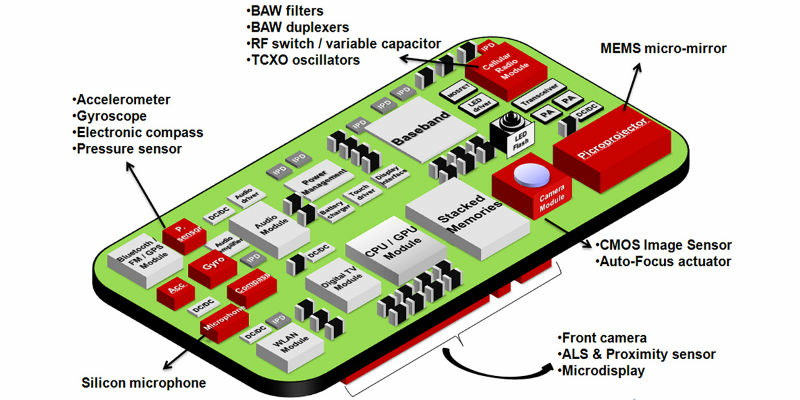
\includegraphics[scale=0.5]{smartphone.png}

{\itshape Source :  flickr / Intel Free Press }
\end{center}



\subsection{Programmation}


\begin{center}
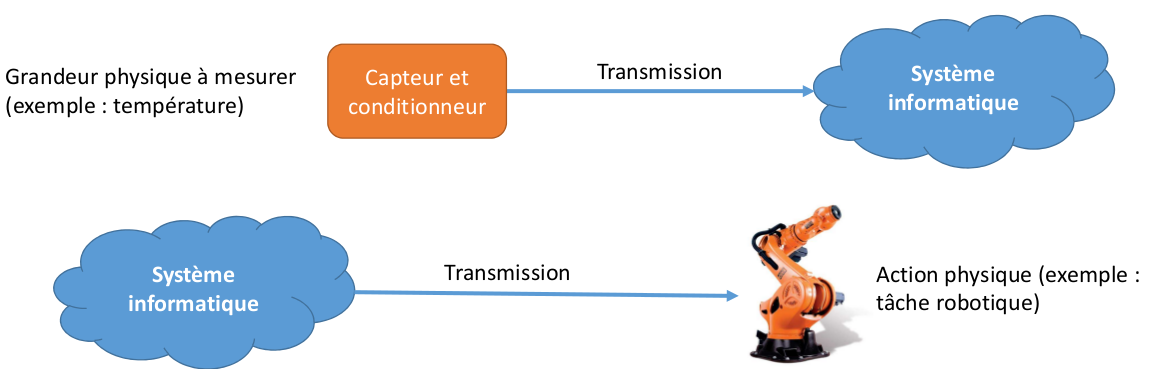
\includegraphics[scale=0.4]{systeme_embarque.png}

{\itshape \small Source : Yassine Haddab Université de Montpellier}
\end{center}


\begin{methode}{}
Un algorithme de contrôle  fréquent sur un système informatique embarqué consiste en une boucle infinie où s'enchaînent capture d'événements par les émetteurs, traitement puis action par les actionneurs.  
\begin{lstlisting}[style=compil]
Initialiser les actionneurs à leur position de départ
Tant que Vrai 
	Lire les informations des capteurs
	Traiter ces informations
	Calculer des informations sur les actionneurs
	Transmettre ces informations aux actionneurs
\end{lstlisting}

\end{methode}



\subsection{QCM type E3C2}


\begin{exerciceB2}{}
Pour chaque question, sélectionner l'unique réponse correcte.

\begin{enumerate}
	\item Identifier parmi les éléments suivants celui qui n'est pas un capteur.

\begin{multicols}{2}
\begin{enumerate}
	\item haut-parleur
	\item caméra
	\item accéléromètre
	\item microphone

\end{enumerate}
\end{multicols}
	
	\item Parmi les éléments suivants, lequel est un capteur ?
	
\begin{multicols}{2}
\begin{enumerate}
\item un bouton poussoir
\item un moteur
\item une diode électroluminescente
\item un afficheur à cristaux liquides

\end{enumerate}
\end{multicols}

\item On réalise une petite station météo.

Quel composant est un capteur ?

\begin{multicols}{2}
\begin{enumerate}
\item l'afficheur LCD
\item l'écran de l'ordinateur
\item la LED
\item le thermomètre
\end{enumerate}
\end{multicols}

\item Parmi les dispositifs d'entrée et de sortie suivants, lequel est
uniquement un capteur ?

\begin{multicols}{2}
\begin{enumerate}
\item la diode
\item l'écran tactile
\item le thermomètre
\item le moteur pas à pas

\end{enumerate}
\end{multicols}
\end{enumerate}

\end{exerciceB2}

 
\section{Interface Homme Machine}

\begin{definition}{}
Une \textbf{Interface Homme Machine} est un ensemble de moyens physiques (boutons, manettes) ou logiciels (interface graphique) qui permettent à un humain d'échanger des informations avec une machine.

Les moyens matériels permettant l'interaction sont appelés \textbf{périphériques} : on distingue les \textbf{périphériques d'entrée} ou de \textbf{sortie}. 

\href{https://interstices.info/50-ans-dinteraction-homme-machine-retours-vers-le-futur/}{Douglas Engelbart} est un des pionniers des IHM en informatique avec son système \textit{NLS} qui introduit  la première souris.
\end{definition}



\begin{exerciceB}{}

Compléter la légende de la figure ci-dessous représentant différents composants et périphériques d'un ordinateur :


\begin{center}
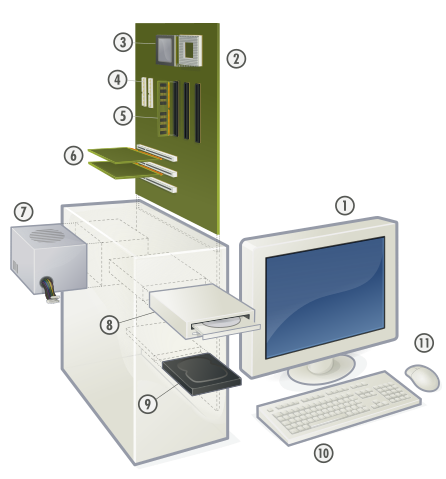
\includegraphics[scale=0.6]{446px-Personal_computer,_exploded_4.svg.png}

\medskip

{\itshape Source : Gustavb / CC BY-SA (http://creativecommons.org/licenses/by-sa/3.0/)}
\end{center}

\end{exerciceB}


\subsection{Fiabilité et sécurité}

\begin{itemize}[label=\ding{43}]

	\item La \textbf{sûreté} est la garantie qu'un système fait ce qu'il doit faire et ne fait pas ce qu'il ne doit pas faire. Les programmes des systèmes embarqués doivent parfois s'exécuter avec des contraintes fortes (manque de ressource, temps de réaction très rapide) et  ils ne sont pas toujours développés avec la rigueur nécessaire. Les bugs sont donc fréquents. Parfois bénins (une mauvaise gestion des années bissextiles a provoqué l'arrêt  du lecteur MP3 Zune de Microsoft le 31/12/2008, ils peuvent avoir  a des conséquences  dramatiques : les bugs  du Therac 25 (appareil de radiographie) ou du contrôle moteur sur les Toyota Camry ont provoqué plusieurs morts.
	
	\item La \textbf{confidentialité} est une problématique majeure des systèmes embarqués qui collectent des données personnelles sur leurs utilisateurs, comme par exemple les cartes électroniques de transport comme le pass Navigoo ou la carte Técély.
	
	\item La \textbf{sécurité}  est souvent un point faible des systèmes embarqués, qui manquent de ressources matérielles, ont des cycles de vie long sans mise à jour et mettent en jeu des modes de communication sans contact particulièrement vulnérables. 
	
Par exemple, une voiture ne peut démarrer que si la carte de démarrage se trouve à proximité car la carte et la voiture partagent un secret commun permettant de déverrouiller le système antidémarrage. \href{https://interstices.info/la-securite-des-systemes-informatiques-ubiquitaires/}{L'attaque par relais} permet  de déjouer ce  protocole  en relayant la communication : un pirate se trouve près de la voiture et l'autre près de la carte et par un leurre technologique ils font croire aux deux parties qu'elles sont à proximité.  Tous les systèmes embarqués qui communiquent sans contact (carte bancaire, carte d'accès \ldots) sont vulnérables à cette attaque.
	
\begin{center}
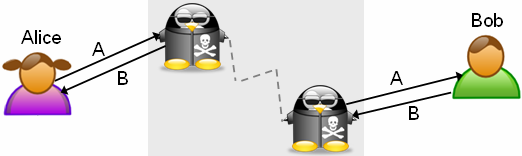
\includegraphics[scale=0.5]{Attaque_par_relais.png}

{\itshape \small Source : Image : Martial Régereau [CC BY-SA 3.0], via Wikimedia Commons}
\end{center}
	
\end{itemize}



\subsection{QCM type E3C2}

\begin{exerciceB2}{}
Pour chaque question, sélectionner l'unique réponse correcte.

\begin{enumerate}
	\item Lequel de ces objets n'est pas un périphérique ?

\begin{multicols}{2}
\begin{enumerate}
	\item le clavier
	\item une clé USB
	\item la carte graphique
	\item la carte mère

\end{enumerate}

\end{multicols}

	\item Lequel de ces périphériques n'est pas un périphérique d'entrée ?

\begin{multicols}{2}
\begin{enumerate}
	\item le moniteur
	\item le clavier
	\item la souris
	\item le scanner

\end{enumerate}

\end{multicols}

\end{enumerate}


\end{exerciceB2}

\section{Objets connectés}

\subsection{Internet des objets}

\vspace*{-20pt}

\begin{definition}{}
Un \textbf{objet connecté} est un système informatique embarqué disposant d'une connexion à un réseau local ou à L'Internet. 

Les Interfaces Homme Machine des objets connectés sont souvent des applications Web disponibles sur Smartphone.


\end{definition}




\begin{center}
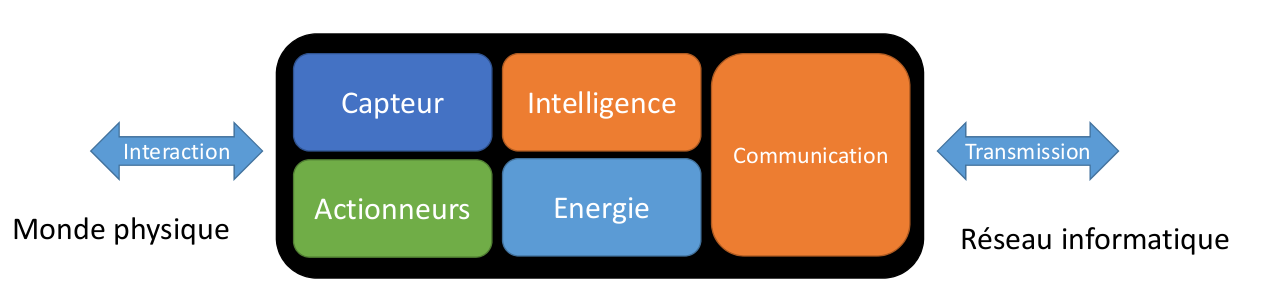
\includegraphics[scale=0.4]{objet-connecte.png}

{\itshape \small Source : Yassine Haddab Université de Montpellier}
\end{center}

Avec la baisse des coûts des microcontrôleurs et des puces Wifi, les objets connectés se multiplient. On peut en fabriquer facilement à partir de cartes Arduino, de Raspberry Pi ou de cartes Wifi ESP8266.
Actuellement, il existe plus d'objets que d'humains connectés à Internet et leur nombre va augmenter fortement dans les prochaines années avec la baisse de coût des . On parle d'\texttt{IOT} pour \href{https://fr.wikipedia.org/wiki/Internet_des_objets}{Internet Of Things} pour désigner l'ensemble des objets connectés à l'Internet.

On estime à 50 milliards le nombre d’objets connectés en 2020.


\subsection{Fiabilité et sécurité}

Les objets connectés permettent d'ajouter de l'intelligence dans notre environnement à tous les niveaux : le corps (mes indicateurs de santé, ma nourriture), la maison(appareils, système de chauffage), les réseaux (électrique, de circulation), les transports (véhicules autonomes), la prévention des risques (incendies) \ldots De plus la collaboration entre objets connectés, leur connexion à des bases de données en ligne, augmente considérablement leur puissance même si chaque objet a des ressources matérielles limitées.

Néanmoins les vulnérabilités des systèmes embarqués sont amplifiées s'ils sont connectés.

\href{https://fr.wikipedia.org/wiki/Cyberattaque_de_2016_contre_Dyn}{La cyberattaque d'un  serveur DNS majeur} par des milliers de caméras de surveillance transformées en bots, a gravement perturbé Internet en Octobre 2016. La prise de contrôle à distance par des hackers de la \href{https://www.wired.com/2015/07/hackers-remotely-kill-jeep-highway/}{Jeep Cherokee} en 2015 ou des failles détectées dans des pacemakers sont des exemples parmi bien d'autres illustrant le fait que la révolution  de l'internet des objets ne pourra se faire sans des progrès sur le plan de leur sécurité.

Enfin  la moisson de données personnelles que  peuvent collecter des objets connectés comme les assistants personnels proposés par les \href{https://fr.wikipedia.org/wiki/GAFAM}{GAFAM}  doit absolument être contrôlée.


\end{document}